\chapter{\textit{Data Warehousing}} 
\label{chap:dw}

	Este capítulo apresenta algumas definições necessárias para que se obtenha uma visão geral de data warehousing e OLAP. Primeiramente é definido o que é um data warehouse e quais são as terminologias relacionadas ao assunto. Em seguida é mostrado as características específicas de um data warehouse, procurando compara-lo aos banco de dados relacionais. Os componentes de um DW são definidos e apresentados e subsequentemente a modelagem que se aplica a um dw é explicitada. Ao final é apresentado a solução de data warehousing para métricas de código-fonte e como ela foi pensada segundo os fundamentos explicados nos tópicos anteriores.

\section{Definições e terminologia}\label{sec:intro}

\citeonline{Inmon1992} define um data warehouse como uma coleção de dados orientada a assunto, integrada, não volátil, variável no tempo para o suporte às decisões da gerência.

\citeonline{hobbs2011oracle} afirma que data warehouse é um banco de dados que contêm dados de múltiplos sistemas que foram consolidados, integrados, agregados e estruturados de modo que que possam ser usados para apoiar o processo de análise e tomada de decisão de um negócio.
 
Os Data Warehouses oferecem armazenamento, funcionalidade e responsividade às consultas além das capacidades dos bancos de dados orientados à transação \cite{elmasri_sistemas_2011}. São vários os tipos de aplicação aceitos para um data warehouse. Algumas delas serão definidas a seguir.


\textbf{OLAP (online analytical processing — processamento analítico on-line)}:
é um conjunto de princípios que fornecem uma estrutura dimensional de apoio à decisão \cite{Kimball2002}. As ferramentas OLAP empregam as capacidades de computação distribuída para análises que requerem mais armazenamento e poder de processamento do que pode estar localizado econômica e eficientemente em um desktop individual \cite{elmasri_sistemas_2011}. Nestas aplicações dados sumariados e históricos são mais importantes que dados atômicos \cite{hilmer2002}.

\textbf{DSS (decision-support systems — sistemas de apoio à decisão)}:
são sistemas que ajudam os principais tomadores de decisões de uma organização com dados de nível mais alto em decisões complexas e importantes \cite{elmasri_sistemas_2011}. Segundo \citeonline{kimball_data_2008}  os DSSs têm como objetivo tornar a informação de uma organização acessível e consistente, prover uma fonte adaptável e resiliente de informações, e garantir a segurança aos dados para assim ser um sistema base para a tomada de decisão.

\textbf{OLTP (online transaction processing) — processamento on-line de transações}:
bancos de dados tradicionais têm suporte para o OLTP, com suas operações de inserção, atualização e exclusão e também à consulta de dados. \citeonline{neeraj_sharma_2011} explica que sistemas OLTP usam tabelas simples para armazenar dados, estes que são normalizados, para se reduzir a redundância ou até mesmo eliminá-los, buscando sempre a garantia de sua consistência.


\section{Características dos data warehouses}\label{sec:caract-dw}


\citeonline{elmasri_sistemas_2011} diferencia um Data warehouse de uma estratégia de multibancos de dados afirmando que o primeiro possui um armazenanento em um modelo multidimensional, assim dados de múltiplas fontes são integrados e processados para tal e sendo assim contrário ao segundo, que oferece acesso a bancos de dados disjuntos e normalmente heterogêneos. 
% comentario Tomioka
A vantagem aqui se nota pela adoção de um padrão de design mais conciso, que pode levar a uma menor complexidade de implantação.

Diferentemente da maioria dos banco de dados transacionais, data warehouses costumam apoiar a análise de série temporal e tendência, ambas exigindo mais dados históricos do que geralmente é mantido nos bancos de dados transacionais \cite{elmasri_sistemas_2011}.

Em comparação com os bancos de dados transacionais, os data warehouses são não-voláteis \cite{elmasri_sistemas_2011}. Sendo assim, suas informações possuem a caracterísca de mudarem de uma forma muito menos frequente, portanto dificilmente seria enquadrada como uma informação em tempo real, e sim como uma de atualização periódica.

Segundo \citeonline{elmasri_sistemas_2011} data warehouses são otimizados para recuperação de dados, e não para processamento de rotina, uma característica intrísica à sistemas OLTP.


% @Características diferenciadoras

\citeonline{elmasri_sistemas_2011} ordena as seguintes características diferenciadoras de data warehouses, proveniente da lista original de \citeonline{codd1993providing} sobre OLAP:

\begin{easylist}[itemize]

& Visão conceitual multidimensional.

& Dimensionalidade genérica.

& Dimensões e níveis de agregação ilimitados.

& Operações irrestritas entre dimensões.

& Tratamento dinâmico de matriz esparsa.

& Arquitetura de cliente-servidor.

& Suporte para múltiplos usuários.

& Acessibilidade.

& Transparência.

& Manipulação de dados intuitiva.

& Desempenho de relatório consistente.

& Recurso de relatório flexível.

\end{easylist}

% @Componentes de um DW

\subsection{Componentes Básicos de um Data Warehouse}

A figura \ref{fig:elem-bas-dw} representa a estrutura básica de um DW segundo \citeonline{Kimball2002}, os componentes serão definidos a seguir.

% @Figure elem-bas-dw
\begin{figure}[h!]
\centering
\includegraphics[keepaspectratio=false,scale=0.53]{figuras/figuras_pedro/elem-bas-dw.eps}
\caption{Elementos básicos de um data warehouse}
\label{fig:elem-bas-dw}
\end{figure}
\FloatBarrier

\textbf{Sistemas de Fonte de Dados Operacionais (OSS - \textit{Operational Source Systems})}:
Representa os sistemas que irão prover informações para o DW. Seus dados podem ser provenientes de outros sistemas OLTPs, planilhas e etc, que compoêm o negócio a ser tratado. Devem ser pensados como fora do data warehouse porque, temos pouco ou nenhum controle sobre o conteúdo e formato dos dados presentes nestes tipos de sistemas legados \cite{Kimball2002}.

\textbf{Área de Preparação dos Dados (DSA - \textit{Data Staging Area})}:
É onde irá ocorrer a possível limpeza e reformatação dos dados antes que sejam carregados no \textit{data warehouse} \cite{elmasri_sistemas_2011}, processo esse conhecido como extração transformação e carga (ETL).

O passo de extração consiste em ler os dados das 
% @termo
fontes operacionais
e copiar o que for necessário para o DW na área de preparação dos dados.

Transformação é o passo que irá tratar os dados agora presente na área de preparação dos dados. Segundo \citeonline{Kimball2002} 
existem diversos tipos de transformações que podem ocorrer, como a limpeza dos dados (correção de erros ortográficos, resolução de dados conflitantes com o domínio, tratamento de dados que estão em falto, ou o 
% @termo
\textit{parse}
de dados para um certo padrão), e também ações como combinar dados de várias fontes, e por fim pode-se atribuir chaves para os dados que irão para o DW.

O terceiro passo do processo de ETL, a carga, é onde os dados que foram tratados, limpo, transformados e padronizados dentro da área de preparação dos dados serão carregados nas tabelas do data warehouse.

\textbf{Área de Apresentação dos dados (DPA - \textit{Data Presentation Area})}:
Representa a área onde os dados são organizados, armazenados e disponibilizados para consulta direta pelos usuários, autores de relatórios, e outras aplicações. Os dados da área de apresentação devem ser dimensionais e atômicos e devem estar de acordo com a arquitetura do DW \cite{Kimball2002}.

% @todo explicar Ferramentas de Acesso de dados 

\textbf{Ferramentas de Acesso de dados (DAT - \textit{Data Access Tools})}:

\textbf{Metadados}: Definido como toda a informação no ambiente de data warehouse que não são os dados em si \cite{Kimball2002}. Os metadados num ambiente DW podem apontar para dados sobre tabelas do sistema, índices, relacionamentos, e etc. \citeonline{kimball1998data} recomenda que a arquitetura de um DW seja orientada a metadados, devido a seu papel crítico de prover informações e parâmetros que permitem que as aplicações executarem suas tarefas com um controle maior sobre os dados provenientes das fontes de dados e outros elementos fundamentais para sua execução.


\section{Modelagem de dados para data warehouses}\label{sec:modelagem-dw}

Modelos multidimensionais tiram proveito dos relacionamentos inerentes nos dados para preencher os dados em matrizes multidimensionais, chamadas cubos de dados \cite{elmasri_sistemas_2011}.

Uma planilha simples contendo uma matriz bidimensional poderia representar as vendas regionais por produto para um determindo período (Figura \ref{fig:bidimensional-dw}). Poderia então ser acrescentado a dimensão de tempo para a relação, assim teríamos o trimestre fiscal para os produtos da região. Isto produziria uma matriz tridimensional, representada por um cubo (Figura \ref{fig:cubo-dw}).


% @Figure bidimensional-dw
\begin{figure}[h!]
\centering
\includegraphics[keepaspectratio=false,scale=0.65]{figuras/figuras_pedro/bidimensional.eps}
\caption{Uma matriz bidimensional}
\label{fig:bidimensional-dw}
\end{figure}
\FloatBarrier


% @Figure cubo-dw
\begin{figure}[h!]
\centering
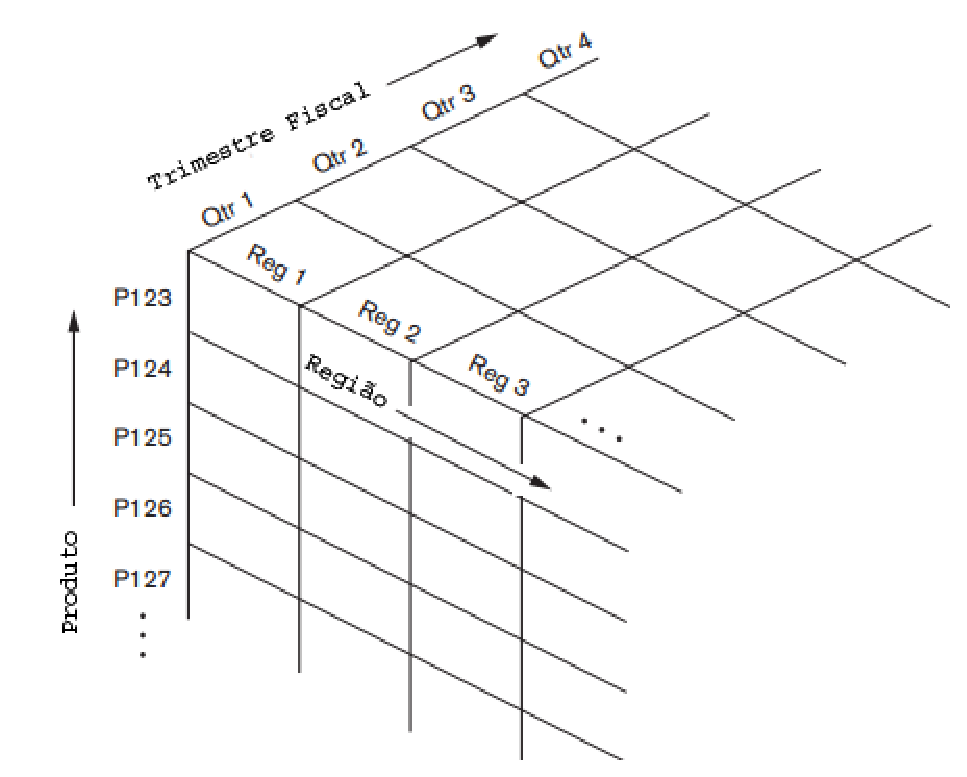
\includegraphics[keepaspectratio=false,scale=0.65]{figuras/figuras_pedro/cubo.eps}
\caption{Um cubo de dados tridimensiona adaptado de \citeonline{elmasri_sistemas_2011}}
\label{fig:cubo-dw}
\end{figure}
\FloatBarrier

O cubo da Figura \ref{fig:cubo-dw} organiza os dados de produto por trimestres fiscais e por região. Cada célula representa a venda de um certo produto, num certo trimestre fiscal em uma certa região. Assim a modelagem permite adicionar mais dimensões, criando-se um hipercubo que combinaria todas as outras anteriores, o único problema é que não seria facilmente visualizada a sua forma gráfica. Porém diversas ferramentas de acesso de dados são capazes de apresentar tais dimensões de acordo com a escolha de combinação do usuário.

As operações possíveis de serem aplicadas a um cubo OLAP são:

\begin{easylist}[itemize]

& \textbf{Pivoting}: Também conhecido como \textit{rotation} (rotação), nessa técnica, o cubo de dados pode ser imaginado girando para mostrar uma orientação diferente dos eixos \cite{elmasri_sistemas_2011}.


& \textbf{Roll-up}: \textit{Drilling} em modelagem multidimensional significa ir de um nível hierárquico a outro \cite{ballard_dimensional_2006}. Portanto \textit{roll-up} ou \textit{drill-up} consiste em subir na hierarquia, agrupando em unidades maiores ao longo de uma dimensão \cite{elmasri_sistemas_2011}.

& \textbf{Drill-Down}: É o inverso de \textit{roll-up}, busca alcançar a informação em um nível maior de detalhamento quanto a sua dimensão.


& \textbf{Slice}: Termo usado para definir um membro ou um grupo de membros que será separado, \textit{Slice}, (de todas as outras dimensões) e em seguida, avaliado através de todas as outras dimensões \cite{ballard_dimensional_2006}.

& \textbf{Dice}: Similar ao \textit{slice}, \citeonline{ballard_dimensional_2006}  caracteriza que esta operação busca combinar membros de diferentes dimensões a partir da escolha de um ou mais membros de uma mesma dimensão, para que assim a interrelação entre elas possa ser analizada.


\end{easylist}

\subsection{Tipos de tabelas do modelo multidimensional}

O modelo multidimensional apresenta dois tipos de tabelas: a tabela de dimensão e fato. Uma tabela de dimensão contém os descritores textuais do negócio \cite{Kimball2002}, ou seja, consiste em tuplas de atributos da dimensão \cite{elmasri_sistemas_2011}. Uma tabela de fato possui tuplas para cada fato registrado. Um fato é uma medida de desempenho do negócio, tipicamente numérico e aditivo \cite{Kimball2002}. Assim a tabela de fatos contém também as dimensões que são indicadas pelos fatos, isto é representado por ponteiros para tabelas de dimensão (um para cada variável de fato observado).

\subsection{Esquemas multidimensionais}

Dois esquemas comuns são o esquema estrela e o esquema floco de neve. O esquema estrela consiste em uma tabela de fatos com uma única tabela para cada dimensão (Figura \ref{fig:star-schema}) \cite{elmasri_sistemas_2011}. O esquema floco de neve é resultado da normalização e expansão das tabelas de dimensão do esquema estrela \cite{ballard_dimensional_2006} (Figura \ref{fig:snowflake}). Segundo \citeonline{Kimball2002} o floco de neve não é recomendado em uma ambiente de data warehouse, pois quase sempre faz com que a apresentação dos dados ao usuário seja mais complexa, além do impacto negativo que causa sobre o desempenho da navegação.

% @Figure star-schema
\begin{figure}[h!]
\centering
\includegraphics[keepaspectratio=false,scale=0.65]{figuras/figuras_pedro/star-schema.eps}
\caption{Um esquema estrela}
\label{fig:star-schema}
\end{figure}
\FloatBarrier

% @Figure snowflake
\begin{figure}[h!]
\centering
\includegraphics[keepaspectratio=false,scale=0.50]{figuras/figuras_pedro/snowflake.eps}
\caption{Um esquema floco de neve}
\label{fig:snowflake}
\end{figure}
\FloatBarrier

\section{Solução de \textit{Data Warehousing} para Métricas de Código-Fonte}

Seguindo a metodologia de \citeonline{Kimball2002} para projetar um data warehouse, \citeonline{rego_monitoramento_2014} projetou uma solução de data warehousing para métricas de código-fonte seguindo quatro passos da metodologia, definidos em cada sub-seção a seguir.


\subsection{Seleção do processo de negócio}

\citeonline{rego_monitoramento_2014} buscou indentificar os processos de negócio e seus respectivos requisitos. Assim foram levantados 15 requisitos de negócio, sendo que os 8 primeiros se referem a avaliação dos valores percentis das métricas de código-fonte e o restante a avaliação de cenários de limpeza e taxa de aproveitamento de oportunidades de melhoria de código-fonte. Os requisitos levantados por \citeonline{rego_monitoramento_2014} foram os seguintes:

\textbf{RN1:}  Visualizar o intervalo qualitativo obtido para cada métrica de código-fonte em uma determinada release do projeto para a configuração \textit{Open JDK8 Metrics}.

\textbf{RN2:}  Comparar o intervalo qualitativo obtido para cada métrica de código-fonte ao longo de todas as releases de um projeto para a configuração \textit{Open JDK8 Metrics}.

\textbf{RN3:}  Visualizar o o valor pecentil obtida para cada métrica de código-fonte em uma determinada release do projeto para a configuração  \textit{Open JDK8 Metrics}.

\textbf{RN4:}  Comparar o o valor pecentil a para cada métrica de código-fonte ao longo de todas as releases para a configuração \textit{Open JDK8 Metrics}.

\textbf{RN5:}  Visualizar o intervalo qualitativo obtido para cada métrica de código-fonte em uma determinada release do projeto para a configuração \textit{Tomcat Metrics}.

\textbf{RN6:}  Comparar o intervalo qualitativo obtido para cada métrica de código-fonte ao longo de todas as releases de um projeto para a configuração \textit{Tomcat Metrics}.

\textbf{RN7:}  Visualizar a medida obtida para cada métrica de código-fonte em uma determinada release do projeto para a configuração \textit{Tomcat Metrics}.

\textbf{RN8:}  Comparar o valor percentil obtido para cada métrica de código-fonte ao longo de todas as releases para a configuração \textit{Tomcat Metrics}.

\textbf{RN9:}  Visualizar a quantidade de cenários de limpeza identificados por tipo de cenários de limpeza de código-fonte em cada classe ao longo de cada \textit{release} de um projeto.

\textbf{RN10:}  Comparar a quantidade de cenários de limpeza por tipo de cenários de limpeza de código-fonte em uma release de um projeto.

\textbf{RN11:}  Visualizar o total de cenários de limpeza em uma determinada release de um projeto.

\textbf{RN12:}  Visualizar cada uma das classes com um determinado cenário de limpeza de código-fonte ao longo das \textit{releases} do projeto.

\textbf{RN13:}  Visualizar as 10 classes de um projeto com menor número de cenários de limpeza identificados.

\textbf{RN14:}  Visualizar as 10 classes de um projeto com maior número de cenários de limpeza identificados.

\textbf{RN15:}  Acompanhar a Taxa de Aproveitamento de Oportunidades de Melhoria de Código-Fonte que é a divisão do  total de cenários de limpeza identificados em uma release e o o número total de classes da mesmarelease de um projeto.


\subsection{Verificação da periodicidade de coleta de dados}

A identificação da periodicidade de coleta dos dados é essencial para que esta seja
realizada de maneira correta, além de viabilizar a agregação dos dados em níveis ou
hierarquias \cite{rego_monitoramento_2014}. Assim a peridicidade foi identificada como as \textit{releases} do software.

\subsection{Identificação dos fatos e das dimensões}

\citeonline{rego_monitoramento_2014} identificou os fatos e dimensões a partir dos termos mais relevantes dos requisitos de negócios levantados. O relacionamento entre fato, natureza do fato e dimensão se mostra na Tabela \ref{tab:dimensoes-fato}.


% @tab:dimensoes-fato
\begin{table}[h]
\centering
\input{tabelas/tabelas-pedro/dimensoes-fato.ltx}
\caption{Fatos e Dimensões do \textit{Projeto de Data Warehouse} por \citeonline{rego_monitoramento_2014}}
\label{tab:dimensoes-fato}
\end{table}
\FloatBarrier

Assim \citeonline{rego_monitoramento_2014} elaborou o modelo físico para o data warehouse:

% @Figure project-dw
\begin{figure}[h!]
\centering
\includegraphics[keepaspectratio=true,scale=0.49]{figuras/figuras_pedro/modelo-dw.eps}
\caption{Projeto Físico do \textit{Data Warehouse} por \citeonline{rego_monitoramento_2014}}
\label{fig:project-dw}
\end{figure}
\FloatBarrier


\citeonline{rego_monitoramento_2014} criou uma área de metadados para facilitar o processo de ETL. A Figura \ref{fig:metadados} mostra a modelagem dos metadados com suas chaves, atributos e relacionamentos. A tabela ``Meta\_Metric\_Ranges'' contém os intervalos qualitativos para cada um das métricas de código-fonte. A tabela ``Meta\_Scenario'' contém os cenários de limpeza do código-fonte e também as recomendações de limpeza para cada cenário de limpeza previsto.

 A tabela  ``Meta\_Metric\_Ranges\_Meta\_Scenario'' possui duas chaves da tabela ``Meta\_Metric\_Ranges'', pois \citeonline{rego_monitoramento_2014} observou a que cada cenário de limpeza identificado deve conter dois intervalos qualitativos de métricas de código-fonte.


% @Figure metadados
\begin{figure}[h!]
\centering
\includegraphics[keepaspectratio=true,scale=0.65]{figuras/figuras_pedro/metadados.eps}
\caption{Metadados do Data Warehouse por \citeonline{rego_monitoramento_2014}}
\label{fig:metadados}
\end{figure}
\FloatBarrier

% @sec:Considerações Finais do Capítulo
\section{Considerações finais do Capítulo}

Nesse capítulo foi apresentado os conceitos de \textit{data warehousing} que foram a base teórica para a elaboração da solução de DW de \citeonline{rego_monitoramento_2014}. No próximo capítulo será apresentado o projeto de estudo de caso com seu protocolo, apresentando a questão de pesquisa motivadora do estudo.